The application that we created consists of two main Panels, two optional floating Panels and one hidden Panel. The main two Panels as well as one of the floating Panels, contain all the tools and the algorithms. The other floating Panel, contains information about the Tkinter, and the hidden Panel, is the Parent Panel which help us to change between each Panel without any error.

\subsubsection*{First Panel}
In the First Panel, with some menu option button, we get the input video and the output folder from the user, and when he presses the submit button we start the Algorithm. This procedure is a multi-thread since we wanted one thread to run the algorithm, and at the same time, another would display to the user some information about the current state of the algorithm. We display it into a huge editable and scroll-able entry that we created, and when the algorithm finishes we change the function of the submit button, to change to the second main Panel. When we change a Panel, we kill all the widgets and threads of the current Panel. In the figure below, someone can see the procedure that we described. For more details on the procedure go to Application Workflow. 

\pagebreak

\begin{figure}[h]
	\centering
	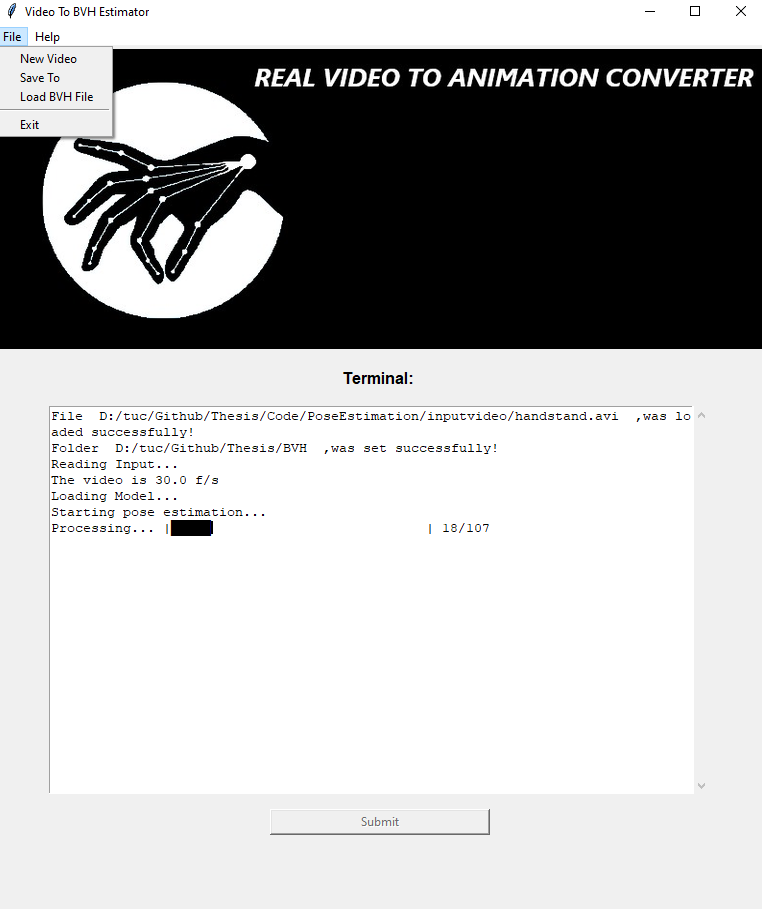
\includegraphics[width=0.7\textwidth]{figures/Implementation/Panel1.png}
	\captionsetup{labelformat=empty}
	\caption{The First Panel of the Application}
\end{figure}

\subsubsection*{Second Panel}
In the second Panel, the user can edit the BVH file that the algorithms in the previous Panel created. We created some separate frames in this Panel. In the first frame, the user can edit the position of the BVH file for each dimension. The way that works, we take the input from each entry space, and we try to cast it to a float. In a false cast, set the value to one, which is considered a neutral input in the multiplication. When the user presses submit, a function that edits for each frame every dimension of the position is being called. Subsequently, the next frame contains the Video Player. This Video  Player loads an mp4 that we create from a BVH file, we discussed it in a previous section. Then it reads some essential information about this mp4, the frame rate, the duration, the size, and some more details, and displays it in a fixed size (700,425) in order to fit and fill the space we left for it in the Application. We give the user the option to play, stop and search through the video with the skip buttons or by moving the video bar. The reset button deletes the current mp4 and creates a new, one with the edited BVH file. This procedure is not very fast, since we have to read the BVH for each frame, create a new 3D space and import the new keypoints location and orientation. For that reason, we give information to the user about the state of that rendering, so while we run that algorithm that converts the BVH file into an mp4 visualization video, we start another thread that displays to the user the frame that the algorithm is now editing. Finally, in this panel, in the menu options, the user can press the BVH filtering which opens a floating Panel that allows the user to smooth with three filters the BVH files and the option to animate another video that returns the user to the first Panel. We also give some information to help the Users by hovering the mouse over the questions marks and some buttons. 

\pagebreak

\begin{figure}[h]
	\centering
	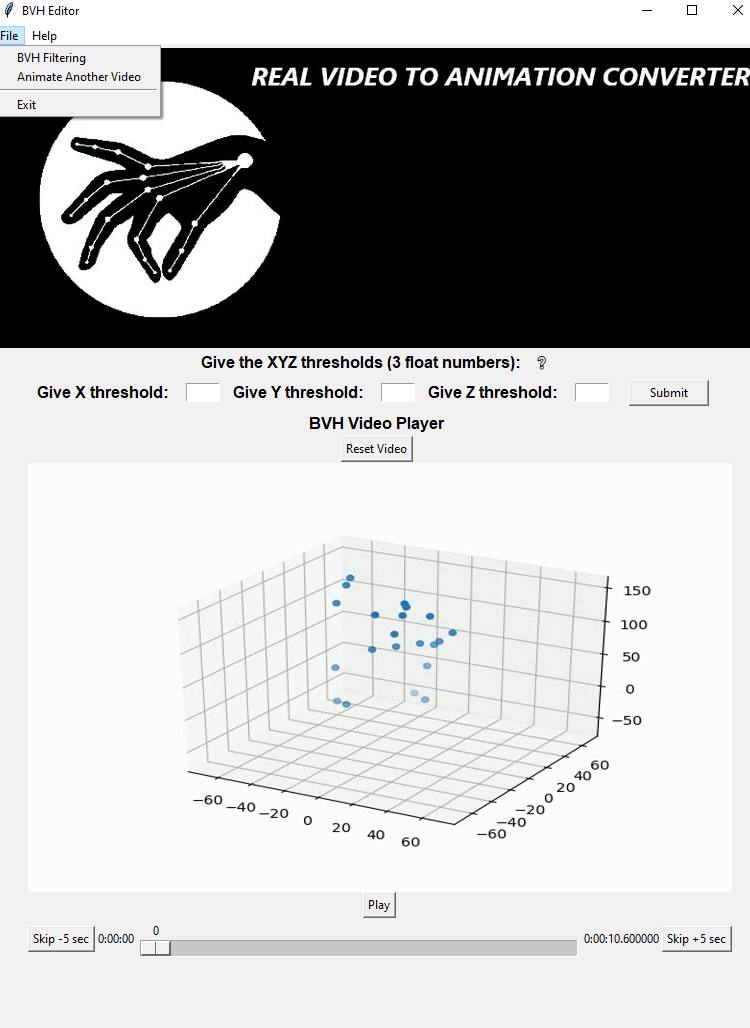
\includegraphics[width=0.7\textwidth]{figures/Implementation/Panel2.png}
	\captionsetup{labelformat=empty}
	\caption{The Second Panel of the Application}
\end{figure}

\subsubsection*{Third Panel}
In this Panel, the user can select between three different filters that remove the Neural networks noise from the BVH file. By hovering the mouse over the question marks we give the user information about these filters. We also suggest some values in the spin-boxes, but we give them the freedom to the user to choose his parameters for each filter. When he presses submit, the filter starts to apply in the BVH file, and when this procedure is complete, a message box confirms it to the user. Then this floating window terminates and the user returns to the second Panel.

\pagebreak

\begin{figure}[h]
	\centering
	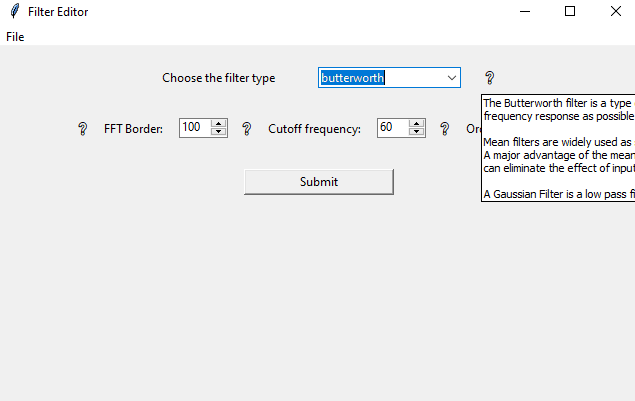
\includegraphics[width=0.7\textwidth]{figures/Implementation/Panel3.png}
	\captionsetup{labelformat=empty}
	\caption{The Third Panel of the Application}
\end{figure}

\subsubsection*{Fourth Panel}
This Panel only gives some information about the Application. It opens when the user presses the About button which is located in the two main Panels, in the Help menu. 

\begin{figure}[h]
	\centering
	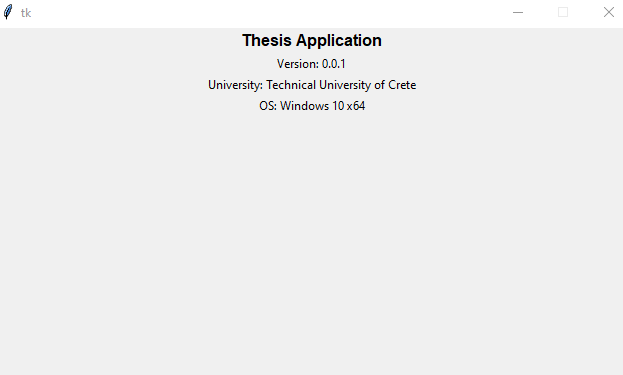
\includegraphics[width=0.7\textwidth]{figures/Implementation/Panel4.png}
	\captionsetup{labelformat=empty}
	\caption{The Fourth Panel of the Application}
\end{figure}

\subsubsection*{Hidden Panel}
The hidden Panel is the Parent Panel that allows us to generate and destroy any other child Panel without killing the Application. Since we do not show anything in this Panel, we made this Panel hidden on purpose